\documentclass[10pt,a4paper]{article}

\usepackage[utf8]{inputenc}
\usepackage[T1]{fontenc}	
\usepackage[italian]{babel}
\usepackage{amsmath}
\usepackage{amsfonts}
\usepackage{amssymb}
\usepackage{graphicx}

\usepackage[left=2cm,right=2cm,top=2cm,bottom=2cm]{geometry}
\geometry{a4paper}

\usepackage{booktabs} % for much better looking tables
\usepackage{verbatim}
\usepackage{subfig} % make it possible to include more than one captioned figure/table in a single 

% pacchetti che mi fanno schifo ma uso lo stesso (Bob è scemo, ma anche Ale...)
\usepackage[cdot, thickqspace, squaren]{SIunits}
% il miglior pacchetto che potessi desiderare
\usepackage{float}
% macro che mi piacciono
\def\code#1{\texttt{#1}}


\title{Esperienza di Franck Hertz}
\author{Gruppo BL \\ Candido Alessandro, Luzio Andrea, Mazziotti Fabrizio}

\begin{document}

\maketitle

\section{Scopo}
Lo scopo di questa esperienza è di verificare la struttura discreta dei livelli energetici degll'atomo di neon e di stimare la sua energia di eccitazione mediante lo studio degli effetti dissipativi negli urti anelastici di elettroni su atomi di neon.

\section{Strumentazione }

\begin{itemize}
 \item Oscilloscopio digitale Tektronix TDS 1012.
 	\begin{itemize}
 		\item Lo strumento è affetto da errore sistematico del 3 \% sulle scale di tensione utilizzate, e di 100 ppm sulle scale di tempo utilizzate.
 	\end{itemize}
 \item Tetrodo a gas neon ELWE U8482230
 \item Sistema di alimentazione e lettura di corrente ELWE

\end{itemize}

\section{Osservazione degli effetti degli urti anelastici elettrone-neon}

Dopo aver eseguito la procedura di accensione suggerita per l'apparato schematizzato in \figurename{~\ref{fig:circuito}},si è osservata la struttura luminosa nel tetrodo a gas al variare delle tensioni $U_{A}$ e $U_{G}$.

\begin{figure}[h!]
	\centering
	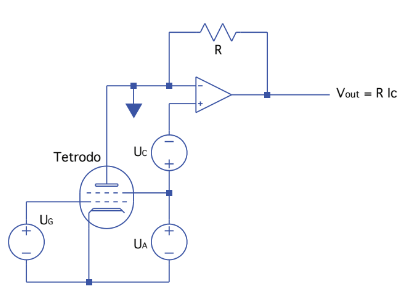
\includegraphics[width=0.80\textwidth]{../grafici/schema_apparato.png}
	\caption{Schema dell'apparato utilizzato nell'esperienza.}
	\label{fig:circuito}
\end{figure}

Come ci si aspetta, mantenendo fisso $U_{G}$ e aumentando la tensione anodica si osserva la comparsa di bande luminose nella parte arancione dello spettro.
Viceversa fissata la tensione anodica e diminuendo $U_{G}$ si ottengono risultati simili, ma l'intervallo su cui è possibile far variare $U_{G}$ è più ristretto (vi sono altre differenze, come descritto nell'Osservazione che segue). In effetti ciò che è rilevante al fine di accelerare gli elettroni è la differenza di potenziale $(U_{A}-U_{G})$, così da permettergli di fare urti anelastici con il neon (cioè per far sì che l'energia degli elettroni sia superiore alla differenza di energia tra due livelli energetici).

\paragraph{Osservazione} La presenza della griglia di controllo permette di definire una superficie equipotenziale, in modo che gli elettroni vengano accelerati come se fossero all'interno di un condensatore a facce piane parallele. Si può notare che diminuendo la tensione ai capi di questa griglia fino a 0, ad un certo punto le bande risultano distorte, in particolare diventando più spesse al centro del tetrodo. Questo è dovuto al fatto che in assenza di potenziale sulla griglia di controllo, il campo elettrico non è proprio uniforme nella regione attraversata dagli elettroni, tranne al più nella zona centrale; ci aspettiamo infatti deviazioni dal comportamento ideale (condensatore infinito) nelle zone periferiche (effetti di bordo).

\paragraph{} Si è fissato $U_{G} = \unit{3.8 \pm 0.1}{V}$, $U_{F}=\unit{8.0 \pm 0.1}{V}$, $U_{E} = \unit{10.6 \pm 0.1}{V}$ \footnote{Per quanto riguarda l'errore su tali misure si veda la Sezione~\ref{errELWE}} e si sono cercate le tensioni $U_{A}$ per le quali compare nelle immediate vicinanze della griglia anodica la prima banda luminosa, la seconda, etc (la tensione frenante $U_E$ è irrilevante perché l'individuazione dei massimi è stata effettuata guardando attraverso la finestra di osservazione e non visualizzando la curva $I_{C}$ vs $U_{A}$ sull'oscilloscopio, ed è quindi indipendente dal comportamento degli elettroni oltre la seconda griglia). La comparsa delle bande corrisponde ai valori massimi della corrente $I_{C}$. Poiché le misure sono state effettuate ad occhio nudo, si sono stimati gli errori su di esse valutando la tensione minima e massima per cui si vedeva la comparsa di una banda. I risultati sono riportati in \tablename{~\ref{tab:massimi}}.

\begin{table}[h!]
\centering
\begin{tabular}{c|c|c|c|c}
\hline
Banda &1&2&3&4\\
\hline 
$U_{A} \unit{}{(\volt)}$ & 22.5 $\pm$ 1.5 & 41.0 $\pm$ 1.5 & 54.5 $\pm$ 1.0 & 72.0 $\pm$ 4.0  \\ 
\hline
\end{tabular}
\captionof{table}{Tensioni $U_{A}$ a fissato $U_{G}$ per cui si osservano comparire le varie bande luminose nelle immediate vicinanze della griglia anodica.}
\label{tab:massimi}
\end{table}


\subparagraph{Differenze} In prima approssimazione ci si aspetta che le differenze fra le tensioni $U_A$ relative a due massimi successivi siano compatibili con l'energia dello stato del neon che che gli elettroni vanno ad eccitare. In tabella sono riportate tali differenze (\tablename{~\ref{tab:differenze}}).

\begin{table}[h!]
	\centering
	\begin{tabular}{c|c|c|c}
		\hline
		Bande (j-i) &1-2&2-3&3-4\\
		\hline 
		$U_{A_i}-U_{A_j} \unit{}{(\volt)}$ & 19 $\pm$ 3  & 13.5 $\pm$ 2.5 & 18 $\pm$ 5\\ 
		\hline
	\end{tabular}
	\captionof{table}{Differenze fra le tensioni in \tablename{~\ref{tab:massimi}}}
	\label{tab:differenze}
\end{table}

La compatibilità fra loro non è ottima, ma non merita ulteriore indagine, infatti la definizione di \emph{comparsa di una banda} è abbastanza ambigua relativamente al fenomeno in esame, per cui gli errori considerati sono evidentemente sottostimati.
%da confrontare con dati andre e valore atteso

\begin{figure}[h!]
	\centering
	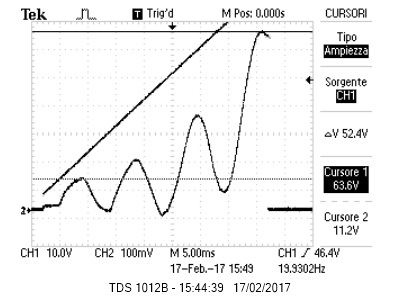
\includegraphics[width=0.80\textwidth]{../oscilloscopio/CorrenteAnodicaTempo1.png}
	\caption{Curva $I_{C} - t$ con rampa per il potenziale $U_{A}$. I valori dei potenziali sono: $U_{F}=\unit{8.0 \pm 0.1}{V}$, $U_{E}=\unit{9.6 \pm 0.1}{V}$, $U_{G}=\unit{3.9 \pm 0.1}{V}$.}
	\label{andamento}
\end{figure}


\subsection{Visualizzazione curva $I_{C}$ vs $U_{A}$ su oscilloscopio}
Si è dunque attivato il generatore di rampa per $U_{A}$ e si è posto l'oscilloscopio in modalità Y-t per osservare la curva $I_{C}$ vs $U_{A}$ (la stessa curva si può osservare in modalità X-Y, dove X = $U_{G}$/10 e Y $\propto I_{C}$, data la linearità della rampa) e la rampa stessa, facendo attenzione a regolare il guadagno dell'OpAmp in modo da non saturarne l'uscita. L'andamento è mostrato in \figurename{~\ref{andamento}}.

\paragraph{} All'aumentare di $U_{A}$, la corrente $I_{C}$ cresce fino a raggiungere un massimo quando l'energia degli elettroni è in grado di eccitare gli atomi di neon(comparsa della prima banda). La presenza del campo frenante dovuto al potenziale $U_{E}$ non permette a questi elettroni, che hanno perso energia in seguito all'urto, di arrivare all'anodo e quindi la corrente registrata diminuisce. la corrente $I_{C}$ ha un minimo quando la banda luminosa si distacca dalla griglia anodica, segno del fatto che gli elettroni hanno perso troppa energia per eccitare di nuovo il neon.
Aumentando ancora $U_{A}$ la corrente reinizia ad aumentare fino a raggiungere un nuovo massimo(comparsa della seconda banda) e così via.

Agendo sulla manopola del potenziale $U_{E}$ si è osservato il variare della curva $I_{C}$ vs $U_{A}$ al variare di $U_{E}$ ottenendo come risultati curve simili alla \figurename{~\ref{andamento}}, come ad esempio quella mostrata in \figurename{~\ref{task6.3}}.
Ci si può aspettare che ci sia una certa distribuzione sull'energia degli elettroni, sia per quelli che hanno fatto urti elastici, sia per gli altri, dovuta principalmente al processo termoionico. All'aumentare di $U_E$ quelli a minore energia non sono più in grado di raggiungere l'anodo con una conseguente diminuzione della corrente anodica.

In \figurename{\ref{task6.3}} il grafico mostrato è proprio quello della curva $I_{C} - U_{A}$ con valori di $U_E$ e $U_G$ tali per cui i minimi sono pressoché allineati sull'asse $I_C = 0$.

Il valore minimo di $U_A$ non è particolarmente rilevante per la ricerca dei massimi, in quanto c'è una zona abbastanza ampia per basse $U_A$ in cui la curva $I_{C} - U_{A}$ è piuttosto piatta, mentre per la tensione massima della rampa si è potuto scegliere il massimo fornito dall'alimentatore, che consente di osservare il quarto massimo, ma non manda in saturazione l'amplificatore opportunamente regolato (si veda ancora \figurename{\ref{task6.3}}).

\begin{figure}[h!]
	\centering
	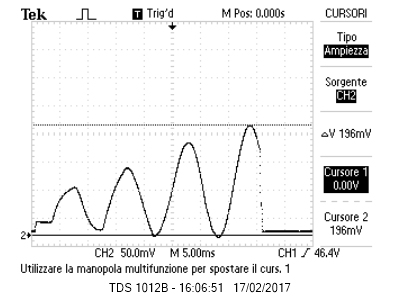
\includegraphics[width=0.80\textwidth]{../oscilloscopio/Task6_3.png}
	\caption{Curva $I_{C} - t$ per $U_{E}=\unit{9.7 \pm 0.1}{\volt}$ e .$U_{G}=\unit{3.5 \pm 0.1}{\volt}$}
	\label{task6.3}
\end{figure}

\section{Note}

\subsection{Sulla stima degli errori del sistema di lettura di corrente ELWE}
\label{errELWE}
Si è ritenuto che l'errore da assumere su tali misure fosse un errore massimo dovuto all'incertezza di lettura (1 digit), supponendo che l'errore statistico fosse trascurabile rispetto a questo.

Infatti la lettura dei valori era stabile nel tempo, e anche osservando i valori di $U_{A, min}$ e $U_{A, max}$ con l'oscilloscopio (inizio e fine rampa) si ha che le fluttuazioni sono dominate dalla discretizzazione.

\subsection{}

%per proseguire da qui in poi servono i valori trovati da Andre (punti 10 e 11)
%si può inserire qualche foto per il punto 9, ma suggerirei di non inerire tutte e 9 quelle buone, ne scegliamo alcune e le affianchiamo
%TODO: si deve inserire gli errori per le tensioni si grafici, cammino libero medio, cose in giro
%ALTRO: decidere le sorti dell'abstract e del commento sulla sensibilità, prendere una decisione su ogni nota che compare


\end{document}